\documentclass[10pt,a4paper]{article}
\usepackage[margin=0.85in]{geometry}
\usepackage{amsmath,amssymb}
\usepackage{graphicx}
\usepackage{booktabs}
\usepackage{enumitem}
\usepackage{float}
\usepackage{hyperref}

\title{\textbf{Introduction to Multimodal Learning: Problem Set 3}\\
\large Motion-Compensated Frame Prediction and Temporal Consistency}
\author{}
\date{}

\begin{document}
\maketitle

\section{Motion-Compensated Frame Prediction (Section 1)}

We use the synthetic clean-translation clip from \texttt{hw3\_utils.py}: a $128\times128$ grayscale sequence in which a $28\times28$ bright square moves with constant velocity $(dy,dx)=(2,4)$ pixels per frame. All five consecutive frame pairs $(t-1,t)$ for $t=1,\dots,5$ are evaluated.

\paragraph{1.1 Previous-frame baseline.} \texttt{frame\_difference} returns $\hat I_t = I_{t-1}$ and $R_t = I_t-I_{t-1}$. Because the square translates uniformly, the absolute residual concentrates on the leading and trailing edges of the square (Fig.~\ref{fig:baseline}), giving MSE $=781.25$, PSNR $=19.20$~dB and residual entropy $0.158$~bits/pixel.

\begin{figure}[H]
    \centering
    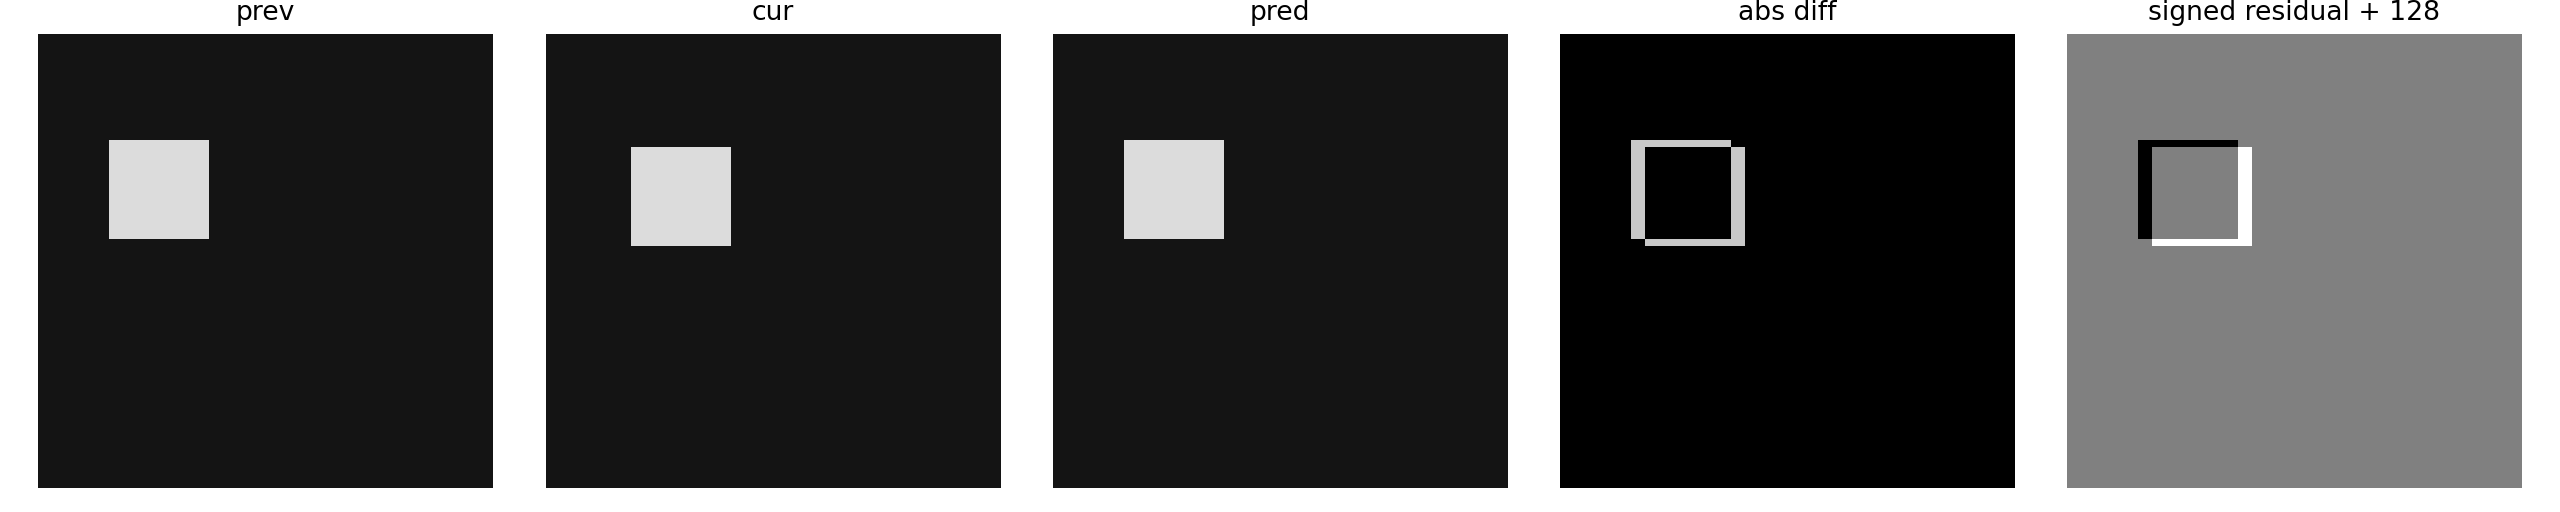
\includegraphics[width=0.85\textwidth]{result/baseline_prediction.png}
    \caption{Previous-frame baseline on $(t{=}0,t{=}1)$. From left to right: $I_{t-1}$, $I_t$, prediction, $|I_t-I_{t-1}|$, signed residual $+128$. The double-edge structure of the absolute residual is the textbook signature of un-compensated translation.}
    \label{fig:baseline}
\end{figure}

\paragraph{1.2 Exhaustive block matching.} \texttt{block\_matching} divides $I_t$ into non-overlapping $B\times B$ blocks and exhaustively searches displacements $(u,v)\in[-R,R]^2$ in $I_{t-1}$, choosing the candidate that minimizes SAD or MSE. The motion field has shape $(H/B,W/B,2)$ with vectors stored as $(dy,dx)$ such that the candidate is taken from $I_{t-1}[y+dy,x+dx]$. Candidates whose top-left falls outside the frame are rejected. The implementation iterates over the $(2R+1)^2$ displacements, gathers all $H_b\!\times\! W_b$ candidate blocks at each shift, computes per-block costs in one tensor pass, and updates the running $\arg\min$ via masked element-wise comparisons.

Table~\ref{tab:bm} averages the four required configurations and the SAD/MSE choice over the five frame pairs of the clean clip. SAD and MSE produce identical motion vectors and identical predictions on this clip (see CSV \texttt{result/block\_matching\_metrics.csv}); we report the SAD column.

\begin{table}[H]
    \centering
    \begin{tabular}{lrrrr}
        \toprule
        Configuration & MSE & PSNR (dB) & H($R_t$) (bits/px) & Runtime (s) \\
        \midrule
        Baseline (frame difference)  & 781.25 & 19.20 & 0.158 & $3.0\!\times\!10^{-5}$ \\
        Block matching $B{=}8,\,R{=}4$  & 0.00 & $\infty$ & 0.000 & 0.019 \\
        Block matching $B{=}16,\,R{=}4$ & 0.00 & $\infty$ & 0.000 & 0.008 \\
        Block matching $B{=}16,\,R{=}8$ & 0.00 & $\infty$ & 0.000 & 0.029 \\
        Block matching $B{=}32,\,R{=}8$ & 365.62 & 22.78 & 0.075 & 0.017 \\
        \bottomrule
    \end{tabular}
    \caption{Mean over five frame pairs (SAD metric). For $B\le16$ the search radius covers the true displacement $(2,4)$, giving exact reconstruction. With $B=32$ a single block straddles the moving square and the static background, so no rigid translation can match it perfectly --- a useful illustration of the block-size/motion-coherence trade-off.}
    \label{tab:bm}
\end{table}

The $B{=}16,R{=}8$ run on $(t{=}0,t{=}1)$ produces motion vectors that are exactly $(-2,-4)$ over every block touching the moving square and $(0,0)$ elsewhere, which is the convention of sampling \texttt{prev[y+dy,x+dx]} for a square that moved by $(+2,+4)$ in frame $t$. The vector field and prediction grids are saved as \texttt{result/block\_b16\_r8\_mv.png} and \texttt{result/block\_b16\_r8\_pred.png} (Fig.~\ref{fig:bm}).

\begin{figure}[H]
    \centering
    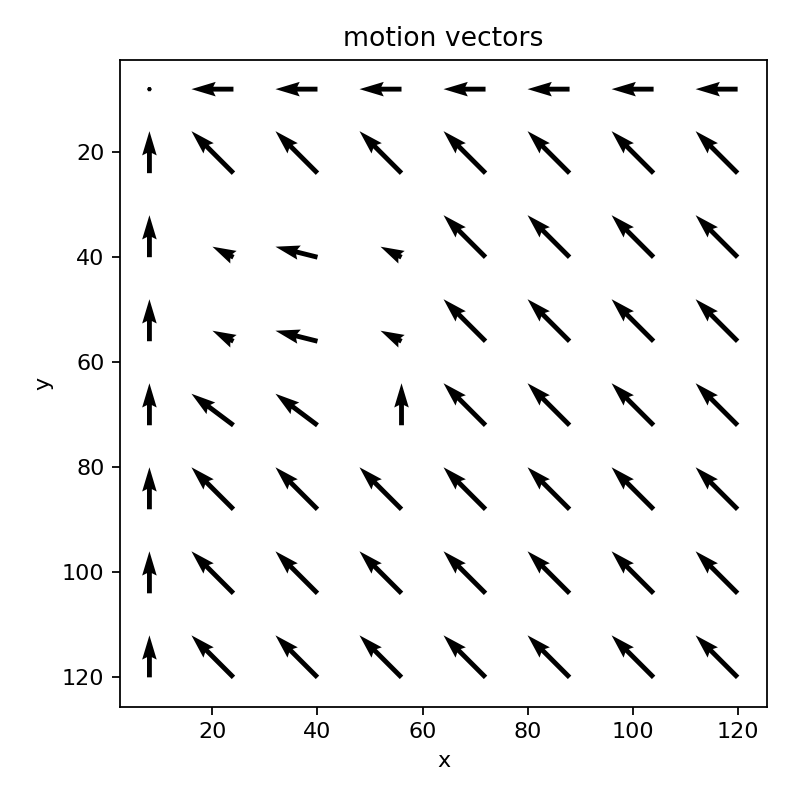
\includegraphics[width=0.27\textwidth]{result/block_b16_r8_mv.png}
    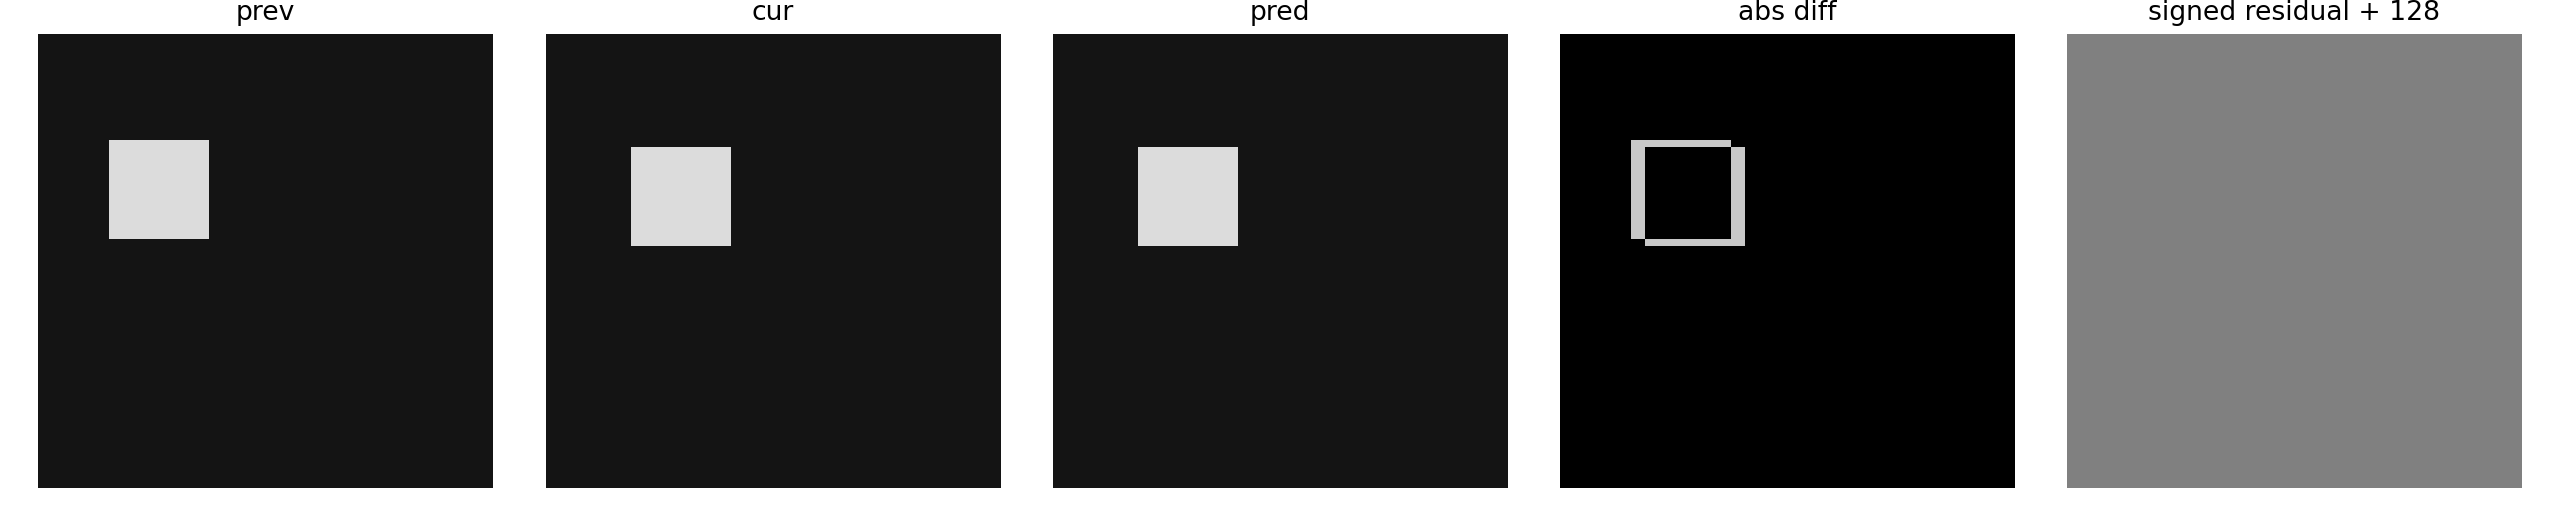
\includegraphics[width=0.55\textwidth]{result/block_b16_r8_pred.png}
    \caption{Block matching with $B{=}16,R{=}8$, SAD. Left: motion-vector field, with non-trivial vectors only on blocks containing the moving square. Right: predicted frame and residual; the residual is identically zero.}
    \label{fig:bm}
\end{figure}

\paragraph{Failure case.} For $B{=}32,R{=}8$ four of the sixteen $32\times 32$ blocks straddle the moving-square / background boundary. Because that boundary is not rigidly translated by any single displacement (only the square is), block matching picks $(0,0)$ for those blocks and the residual concentrates on the leading/trailing edges. PSNR rises to $22.78$~dB versus the baseline's $19.20$~dB but cannot reach perfect reconstruction --- the classical block-size / motion-coherence trade-off.

\section{Temporal Consistency Evaluation (Section 2)}

\paragraph{2.1 Objective metrics.} We implement variance-of-Laplacian sharpness, mean L1 first-order temporal difference, mean L1 second-order temporal acceleration ($\|I_{t+1}-2I_t+I_{t-1}\|_1$), and mean block-motion magnitude (from Section~1, $B{=}16,R{=}8$).

\begin{table}[H]
    \centering
    \begin{tabular}{lrrrr}
        \toprule
        Clip & Sharpness & Temp. diff & Temp. accel & Motion mag (px) \\
        \midrule
        clean\_translation & 566.4 & 3.91 & 7.81 & 9.88 \\
        flicker            & 538.8 & 46.11 & 91.40 & 9.43 \\
        jitter             & 566.4 & 6.43 & 12.97 & 10.05 \\
        blur               &   5.1 & 2.56 & 2.42 & 9.07 \\
        \bottomrule
    \end{tabular}
    \caption{Per-clip objective metrics. Sharpness is variance of Laplacian; temporal-difference and -acceleration are mean L1 over consecutive and three-frame triplets; motion magnitude is mean L2 of block-matching vectors.}
    \label{tab:metrics}
\end{table}

\paragraph{2.2 Human evaluation (1--5 ratings).}
\begin{itemize}[nosep]
    \item \textbf{clean\_translation:} visual\,5, temporal\,5, naturalness\,5 --- clean uniform translation, no visible artifacts.
    \item \textbf{flicker:} visual\,3, temporal\,2, naturalness\,3 --- alternating brightness creates strong flicker between odd/even frames.
    \item \textbf{jitter:} visual\,3, temporal\,2, naturalness\,2 --- non-uniform vertical and horizontal offsets give a visibly shaky look.
    \item \textbf{blur:} visual\,3, temporal\,5, naturalness\,4 --- Gaussian blur reduces sharpness but motion remains smooth.
\end{itemize}

\paragraph{2.3 Discussion.}
\begin{enumerate}[leftmargin=*,itemsep=0pt]
    \item \emph{Best-aligned metric.} Temporal acceleration is the most informative for our human ratings. The flicker clip's score ($91.4$) is an order of magnitude larger than the clean clip ($7.8$) and the jitter clip ($13.0$), exactly matching the perceived ordering by temporal consistency. The first-order temporal difference is also large for flicker but not by as wide a margin, since uniform translation already produces a non-trivial first difference.
    \item \emph{Misleading metric.} Frame sharpness misranks the blur clip: variance of Laplacian collapses to $5.1$, suggesting catastrophic quality, but a human rates the blur clip's \emph{temporal} consistency as $5/5$ because the motion is smooth --- only the spatial frequencies are gone. Sharpness conflates spatial fidelity with overall video quality. Likewise, temporal-difference misleads on the clean clip vs.\ jitter: their first-difference values ($3.9$ vs.\ $6.4$) are close even though humans rank them very differently for temporal consistency.
    \item \emph{Why one scalar is insufficient.} Generated-video quality is multidimensional: spatial fidelity (sharpness, distortion), temporal consistency (flicker, jitter), motion plausibility (smoothness, semantics), and content correctness (subject/text alignment) are largely independent. A single scalar must average over these axes and so masks failure modes --- VBench's design philosophy is exactly this: a panel of axis-specific metrics with separate scores. Two videos with the same averaged score can be perceptually very different (one blurry but smooth, one sharp but flickering), and a single number cannot tell us which.
\end{enumerate}

\section{Short Conceptual Questions (Section 3)}

\subsection*{3.1 Optical-flow constraint}
Brightness constancy: $I(x+u,y+v,t+1)=I(x,y,t)$. First-order Taylor expansion of the LHS around $(x,y,t)$:
\[
    I(x,y,t) + I_x u + I_y v + I_t \cdot 1 + \mathcal{O}(\|(u,v,1)\|^2) = I(x,y,t),
\]
which to first order gives the brightness-constancy / optical-flow equation
\[
    \boxed{\,I_x\,u + I_y\,v + I_t = 0.\,}
\]
\textbf{Under-constrainedness (aperture problem).} This is one scalar equation in two unknowns $(u,v)$ at each pixel. Geometrically the solution lies on a 1D line in flow-space whose normal is $\nabla I=(I_x,I_y)$: only the flow component along the local image gradient (the \emph{normal flow}) is observable, while the component tangent to an isophote --- moving along an edge of constant intensity --- is invisible to the constraint. To recover both components one must add a regularizer (Horn--Schunck), assume local flow constancy and solve a $2\times 2$ system over a window (Lucas--Kanade), or impose higher-order assumptions.

\subsection*{3.2 Space-time attention complexity}
Let $N_s = HW$ tokens per frame, $T$ frames, hidden dimension $d$. We count attention-matrix and projection FLOPs in big-$\Theta$.

\paragraph{(a) Joint space-time self-attention.} All $TN_s = THW$ tokens attend jointly. The attention map is $(THW)\times(THW)$ and the QK$^\top$/softmax/attention$\cdot$V cost is
\[
    \Theta\bigl((THW)^2 d\bigr) = \Theta(T^2 H^2 W^2 d).
\]
QKV projections add $\Theta(THW d^2)$, dominated by the attention term for large $THW$.

\paragraph{(b) Factorized (spatial, then temporal) attention.}
\emph{Spatial}: for each of the $T$ frames, attention over $HW$ tokens costs $\Theta((HW)^2 d)$, summed over frames giving $\Theta(T H^2 W^2 d)$. \emph{Temporal}: at each of the $HW$ spatial positions, attention over $T$ tokens costs $\Theta(T^2 d)$, summed giving $\Theta(HW T^2 d)$. Total
\[
    \Theta\bigl(T H^2 W^2 d + HW T^2 d\bigr) = \Theta\bigl(THW(HW + T)\,d\bigr).
\]

\paragraph{(c) Numerical comparison for $T{=}16, H{=}W{=}32$.}
$THW = 16{\cdot}1024 = 16{,}384$, so joint attention pays $(16384)^2 \approx 2.68\!\times\!10^8$ pairwise scores per head. Factorized: spatial $T(HW)^2 = 16\cdot 1024^2 \approx 1.68\!\times\!10^7$; temporal $HW\cdot T^2 = 1024\cdot 256 \approx 2.62\!\times\!10^5$. The total $\approx 1.7\!\times\!10^7$ is roughly $\mathbf{16\times}$ cheaper than joint, because $HW \gg T$ here so $HW+T\approx HW$ and the saving is exactly the factor $T$. More generally, factorizing avoids the cross-term $T\cdot HW$ inside the attention map and reduces $T^2(HW)^2$ to $T(HW)^2 + (HW)T^2$. Memory for the attention matrix shrinks correspondingly from $\Theta((THW)^2)$ to $\Theta((HW)^2 + T^2)$.

\section{Bonus: Hierarchical Block Matching (Option B)}

We build a 3-level Gaussian pyramid (5-tap kernel $[1,4,6,4,1]/16$ applied separably with reflect padding, then $2\!\times\!$ subsample), run exhaustive block matching at the coarsest level with $R{=}4$, and refine each finer level by upsampling the motion field (vectors $\times 2$, grid $\times 2$) and searching $\pm1$ pixel around the prediction. The effective full-resolution search radius is $4\!\cdot\!4 + 1\!\cdot\!2 + 1 = 19$~px, comparable to the exhaustive $R{=}8$ baseline.

\begin{table}[H]
    \centering
    \begin{tabular}{lrrr}
        \toprule
        Method & Mean PSNR (dB) & Mean MSE & Mean runtime (s) \\
        \midrule
        Exhaustive $B{=}16,R{=}8$       & $\infty$ (perfect) & 0.0  & 0.029 \\
        Hierarchical $B{=}16$, 3 levels & 35.13 & 27.19 & 0.005 \\
        \bottomrule
    \end{tabular}
    \caption{Hierarchical vs.\ exhaustive on five frame pairs of the clean translation clip. Hierarchical search is roughly $\mathbf{6\times}$ faster on $128\!\times\!128$ frames, at the cost of a finite (still high) PSNR. The residual error originates at the coarsest level: after $2\!\times\!$ downsampling the per-frame displacement is only $1$~px, which the integer search rounds; subsequent $\pm1$~px refinement cannot recover sub-block translations on the half-resolution grid where the square boundary is mis-aligned.}
    \label{tab:bonus}
\end{table}

The full per-frame numbers, the hierarchical motion-vector visualization (\texttt{result/hierarchical\_mv.png}) and the prediction grid (\texttt{result/hierarchical\_pred.png}) are saved alongside the exhaustive outputs in \texttt{result/}.

\paragraph{Reproducibility.} Run \texttt{HW3.ipynb} (CPU only, $<1$~min). Outputs are saved to \texttt{result/}: GIFs of the four clips, prediction/motion-vector plots, and CSVs \texttt{block\_matching\_metrics.csv}, \texttt{consistency\_metrics.csv}, \texttt{human\_eval.csv}, \texttt{hierarchical\_vs\_exhaustive.csv}. A sanity check in cell~6 confirms block-matching vectors are exactly $(-2,-4)$ on the moving square, matching the synthetic ground truth.

\end{document}
